\documentclass[oupdraft]{sysbio_sse}
% \usepackage[colorlinks=true, urlcolor=citecolor, linkcolor=citecolor, citecolor=citecolor]{hyperref}
\usepackage{url}

\usepackage{indentfirst}

% Add history information for the article if required
%\history{Received Month X, 20XX;
%revised Month X, 20XX}

\bibliographystyle{plainnat}
\setcitestyle{authoryear,round}
\let\cite\citep

\usepackage{booktabs}
\usepackage[finalizecache,outputdir=manuscript/out,cachedir=manuscript/out/minted-cache]{minted}
\usepackage{multirow}
\usepackage{setspace}
\usepackage[T1]{fontenc}
\setcounter{secnumdepth}{0}
\setminted{baselinestretch=0.9}


\begin{document}

% Title of paper

% Identify the name, address, telephone/fax numbers, and e-mail address for the author who will receive proofs and be designated the "corresponding author" in text.

\title{TreeFlow: Probabilistic Programming and Automatic Differentiation for Phylogenetics
}
% Each important word in the title should begin with a capital letter

% List of authors, with corresponding author marked by asterisk
\author{Christiaan Swanepoel,$^{\ast, 1, 2}$
Mathieu Fourment,$^{3}$
Xiang Ji,$^{4}$
Hassan Nasif,$^{5}$
Marc A Suchard,$^{6,7,8}$
Frederick A Matsen IV,$^{5,9,10}$
Alexei J Drummond$^{1,11}$
\\[4pt]
    % Author addresses
    ${^1}$Centre for Computational Evolution, The University of Auckland, Auckland, New Zealand;\\
$^{2}$School of Computer Science, The University of Auckland, Auckland, New Zealand, 1010;\\
$^{3}$Australian Institute for Microbiology and Infection, University of Technology Sydney, Ultimo NSW, Australia;\\
$^{4}$Department of Mathematics, Tulane University, New Orleans, USA;\\
$^{5}$Public Health Sciences Division, Fred Hutchinson Cancer Research Center, Seattle, Washington, USA;\\
$^{6}$Department of Human Genetics, University of California, Los Angeles, USA;\\
$^{7}$Department of Computational Medicine, University of California, Los Angeles, USA;\\
$^{8}$Department of Biostatistics, University of California, Los Angeles, USA;\\
$^{9}$Department of Statistics, University of Washington, Seattle, USA;\\
$^{10}$Department of Genome Sciences, University of Washington, Seattle, USA;\\
$^{11}$School of Biological Sciences, The University of Auckland, Auckland, New Zealand, 1010;\\
 [2pt]
    % E-mail address for correspondence
    \textit{Correspondence to be sent to: School of Computer Science, The University of Auckland, Auckland, New Zealand, 1010;\\
Email: cswa648@aucklanduni.ac.nz
}}


% Running headers of paper:
\markboth%
% First field is the short list of authors
{Swanepoel et al.}
% Second field is the short title of the paper
{TreeFlow}
% This should be shortened version of the title and no greater than 50 characters

\maketitle

\begin{abstract}
    {Probabilistic programming frameworks are powerful tools for statistical modelling and inference. They are not immediately generalisable to phylogenetic problems due to the particular computational properties of the phylogenetic tree object. TreeFlow is a software library for probabilistic programming and automatic differentiation with phylogenetic trees. It implements inference algorithms for phylogenetic tree times and model parameters given a tree topology. We demonstrate how TreeFlow can be used to quickly implement and assess new models. We also show that it provides reasonable performance for gradient-based inference algorithms compared to specialized computational libraries for phylogenetics.
}
    {phylogenetics; Bayesian inference; probabilistic programming; variational inference}
\end{abstract}
\newline


\section{Introduction}

% Motivate probabilistic programming/phylogenetics
Traditionally, phylogenetic analyses have been performed by specialized software \cite{stamatakis2014raxml, drummond2012bayesian, huelsenbeck2001mrbayes}. A number of software packages exist that implement a broad but predefined collection of models and associated specialized inference methods. Typically, inference is handled by carefully crafted but computationally costly stochastic optimisation or Markov chain Monte Carlo (MCMC) methods \cite{metropolis1953equation, hastings1970monte}. In contrast, in other realms of statistical analysis, \textit{probabilistic programming} software libraries have entered into widespread use. These allow the specification of almost any model as a probabilistic program, and inference is provided automatically with a generic inference method. Exploiting the power of probabilistic programming in phylogenetic analyses could significantly accelerate research by making the process of developing new models and implementing inference faster and more flexible.

% Review probabilistic programming
Probabilistic programming tools, such as BUGS \cite{lunn2000winbugs}, Stan \cite{carpenter2017stan}, PyMC3 \cite{salvatier2016probabilistic}, Pyro \cite{bingham2019pyro}, and TensorFlow Probability \cite{dillon2017tensorflow} allow users to specify probabilistic models by describing the generative process with code as a \textit{probabilistic program}. Advancements in automatic inference methods have allow these tools to perform efficient inference on almost any model. Some notable examples, including automatic differentiation variational inference \cite{kucukelbir2017automatic} (ADVI) and Hamiltonian Monte Carlo \cite{duane1987hybrid} (HMC), use local  gradient information from the model's probability density function to efficiently navigate the parameter space.

One key technology that enables these gradient-based automatic inference algorithms is \textit{automatic differentiation}. Automatic differentiation refers to methods which efficiently calculate machine-precision gradients of functions, specified by computer programs, without extra analytical derivation or excessive computational overhead compared to the function evaluation. Automatic differentiation frameworks that have statistical inference packages built on top of them include Theano \cite{bergstra2010theano}, Pytorch \cite{paszke2019pytorch}, JAX \cite{jax2018github} and TensorFlow \cite{abadi2016tensorflow}. Some of these extend to non-trivial computational constructs such as control flow and recursion \cite{yu2018dynamic}.

The structure of the phylogenetic tree object is a major barrier to implementing probabilistic programming for phylogenetics. It is not clear how the association between its discrete and continuous quantities (the topology and branch lengths respectively) should be represented and handled in inference. Also, the combinatorial explosion of the size of discrete part of the phylogenetic state space presents a major challenge to any inference algorithm. Generic random search methods for discrete variables, as in the naive implementation of MCMC sampling, do not scale appropriately to allow inference on modern datasets with thousands of taxa.

Efforts have already been made to apply probabilistic programming to phylogenetic methods
\cite{fourment2019evaluating, ronquist2021universal, drummond2022linguaphylo}. It has been shown that \textit{universal probabilistic programming languages}, a particularly expressive extension of the class of traditional probabilistic programming languages, can be used to express generative processes for trees, and use them to generate Sequential Monte Carlo inference schemes for complex speciation models \cite{ronquist2021universal}. Another tool, LinguaPhylo, provides a domain specific modelling language for phylogenetics and has the capability to generate a specification for an MCMC sampler for inference \cite{drummond2022linguaphylo}. These approaches both potentially lack the inherent scalability that the automatic inference methods that accompany general-purpose probabilistic modelling tools provide.

Applying scalable inference methods to phylogenetics is a major challenge. \textit{Probabilistic path Hamiltonian Monte Carlo} has been developed to use gradient information to sample phylogenetic posteriors across multiple tree topologies \cite{dinh2017probabilistic}, though moves between tree topologies are not totally informed by gradient information and are similar to the random-walk proposal distributions available to standard MCMC routines. Hamiltonian Monte Carlo proposals for continuous parameters within tree topologies has been paired with standard MCMC moves between topologies for estimating local mutation rates and divergence times using scalable algorithms for gradient calculation \cite{ji2021scalable, fisher2021shrinkage}. Another approach has used Stan to apply automatic differentiation variational inference to phylogenetic inference within a fixed rooted tree topology \cite{fourment2019evaluating}. Finally, variational inference has been applied to phylogenetic tree inference using a clade-based distribution on unrooted tree topologies \cite{zhang2018variational}. This approach has been extended to a more expressive family of approximating distributions \cite{zhang2020improved}, and applied to rooted phylogenies \cite{zhang2022variational}.

One core computation that presents a challenge to automatic differentiation is the \textit{phylogenetic likelihood} \cite{felsenstein1981evolutionary}. This computes the probability function of a collection of sequences given a phylogenetic tree, integrating out the character states at ancestral nodes. This is most efficiently performed through dynamic programming, which requires sequential control flow or recursion, and thus can be non-trivial to implement in a functional automatic differentiation framework such as TensorFlow. Additionally, since the computational cost scales linearly with the number of sequences, naively computing the likelihood's gradient with respect to each branch of the tree yields a quadratic computational cost \cite{ji2020gradients}.

\section{Software Description}

\subsection{Trees and Tensors}

TreeFlow is a library for probabilistic programming in Python. It is built on TensorFlow, a computational framework for machine learning. TreeFlow leverages TensorFlow's capabilities for accelerated numerical computation and automatic differentiation. It uses the existing probabilistic modelling infrastructure provided by TensorFlow Probability, which implements standard statistical distributions and inferential machinery \cite{dillon2017tensorflow}. TreeFlow provides a phylogenetic tree representation for TensorFlow and associated input and output methods, a range of widely used phylogenetic distributions and functions, and tools for applying modern statistical inference methods to phylogenetic models.
% TODO: Flesh out this first paragraph

TensorFlow's core computational object is the Tensor, a multi-dimensional array with a uniform data type. Phylogenetic trees are not immediately at home in a Tensor-centric universe, as they are a complex data structure, often defined recursively, with both continuous and discrete components. TreeFlow represents trees as a structure of Tensors; floating point Tensors representing the times and branch lengths, and integer Tensors representing the topology. The topological Tensors include indices of node parents, children, and for pre- and post-order traversals. TensorFlow has extensive support for `nested' structures of Tensors, including using them as arguments to compiled functions and defining distributions over complex objects. This means computations and models involving phylogenetic trees can be expressed naturally.

A range of phylogenetic distributions and models are implemented in TreeFlow. These are primarily generative models for phylogenetic trees and models of molecular sequence evolution. Generative models of phylogenetic trees, such as Kingman's coalescent \cite{kuhner1995estimating} and Birth-Death-Sampling speciation processes \cite{stadler2009incomplete}, can be used to infer parameters related to population dynamics from genetic sequence data. TreeFlow implements models of nucleotide sequence evolution such as the Jukes-Cantor \cite{jukes1969evolution}, HKY85 \cite{hasegawa1985dating}, and General Time Reversible (GTR) \cite{tavare1986some} models. It includes a standard approach for dealing with heterogeneity in mutation rate across sites based on a marginalizing over a discretized site rate distribution \cite{yang1994maximum}. The probabilistic programming framework, however, allows for the use of any appropriate distribution as the base site rate distribution rather than just the standard single-parameter Gamma distribution. For example, it is straightforward to replace the base Gamma distribution with a Weibull distribution, which has a quantile function that is much easier to compute \cite{fourment2019evaluating}. Thanks to TensorFlow's vectorized arithmetic operations, it is also natural to model variations in mutation rate over lineages by specifying parameters for multiple rates (possibly with a hierarchical prior) and multiplying by the branch lengths of the phylogenetic (time) tree. Models which can be naturally expressed this way include the log-Normal random local clock \cite{drummond2006relaxed} and auto-correlated relaxed clock models \cite{thorne1998estimating}.

% Phylogenetic likelihood 
A computation that requires special treatment is the \textit{phylogenetic likelihood}, the probability of a sequence alignment given a phylogeny and model of sequence evolution. This typically involves integrating out character states at unsampled ancestral nodes using a \textit{dynamic programming} computation known as \textit{Felsenstein's pruning algorithm} \cite{felsenstein1981evolutionary}. The postorder tree traversal and dynamic data structure are not obviously compatible with TensorFlow's immutable data structures and focus on vectorized computations. Additionally, naive implementations result in gradient computations with problematic scaling. The computational cost of computing the derivatives of this likelihood with respect to all the branches of the phylogenetic tree could grow quadratically with respect to the number of taxa, and would prohibit gradient-based inference on large datasets \cite{ji2020gradients}. These issues are overcome in TreeFlow by implementing the dynamic programming data structure with TensorFlow's TensorArray construct \cite{yu2018dynamic}. The TensorArray is a data structure representing a collection of tensors which allows efficient implementation of the sequential computation. The \textit{write-once} property enforced on its constituent tensors ensures that gradient computations have appropriate scaling, as evidenced by benchmarks (see Figure \ref{fig:benchmark}).

% Ratio transform
Another useful tool for phylogenetic inference implemented in TreeFlow is the \textit{node height ratio transform} \cite{kishino2001performance}. This has been used to infer times on phylogenetic trees using maximum likelihood in the PAML software package \cite{yang2007paml}. The ratio transform parametrizes the internal node heights of a tree as the ratio between a node's height and its parent's height. The heights can be computed from the ratios in a pre-order tree traversal. This transformation has a triangular Jacobian matrix, which means computing the determinant required for change of variable of a probability density can be computed in linear time with respect to the number of internal node heights \cite{fourment2019evaluating}. In combination with a log transformation of the root height and a logit transformation of the ratios, a multivariate distribution that takes real values can be transformed into a distribution on internal node heights of rooted phylogenies. This has been applied to Bayesian phylogenetic inference in the context of automatic differentiation variational inference \cite{fourment2019evaluating} and Hamiltonian Monte Carlo \cite{ji2021scalable}. The ratio transform is implemented using a TensorArray-based computation as a TensorFlow Probability Bijector which provides a convenient interface for transforming real-valued distributions into phylogenetic tree distributions.

TensorFlow Probability distributions can be composed into a \textit{probabilistic graphical model} using TensorFlow Probability's joint distribution functionality \cite{piponi2020joint}. The code to specify a joint distribution provides a concise representation of the model used in a data analysis. The ability to implement phylogenetic models in this framework means that automatic inference algorithms implemented in TensorFlow can be leveraged. The discrete topology element of phylogenetic trees is an obstacle in the usage of these algorithms, which are typically restricted to continuous latent variables. Often, the phylogenetic tree topology is not the latent variable of interest, and is not a significant source of uncertainty \cite{yang2000codon}. This can be the case when divergence times or other substitution or speciation model parameters are the focus. In this scenario, useful results can be obtained by performing inference with a fixed tree topology, such as one obtained from fast maximum likelihood methods. This is the approach taken by the NextStrain platform \cite{hadfield2018nextstrain}, which uses the scalability afforded by a fixed tree topology to allow large-scale rapid phylodynamic analysis of pathogen molecular sequence data.

\subsection{Variational inference}

% Inference
One form of statistical inference for which the gradient computation is essential is variational Bayesian inference \cite{jordan1999introduction}. The goal of Bayesian inference is to characterise a \textit{posterior distribution} which represents uncertainty over model parameters. Variational Bayesian inference achieves this by optimizing an approximation to the posterior distribution which has more convenient analytical properties. Typically, the optimisation routine used in variational inference can scale to a larger number of model parameters than the random-walk sampling methods used by MCMC methods.

One concrete implementation of variational inference is \textit{automatic differentiation variational inference} (ADVI) \cite{kucukelbir2017automatic}. ADVI can perform inference on a wide range of probabilistic graphical models composed of continuous variables. It automatically constructs an approximation to the posterior by transforming a convenient base distribution to respect the domains of the model's component distributions. It then optimizes this approximation using stochastic gradient methods \cite{robbins1951stochastic, bottou2010large}. Typically, independent Normal distributions are used as the base distribution for computational convenience. This is known as the \textit{mean field approximation}, and for posterior distributions that have significant correlation-structure, skew, multi-modality, or heavy tails, can introduce error in parameter estimation \cite{blei2017variational}. Possible solutions to this approximation error include highly flexible variational approximations with large numbers of parameters \cite{rezende2015variational} or structured approximations that are informed by the form of the model \cite{ambrogioni2021automatic}.

TreeFlow implements ADVI using TensorFlow Probability's bijector framework to transform a base distribution and leverages the stochastic gradient optimizers already implemented in TensorFlow. Tree variables are estimated by fixing the topology. The base distribution for the divergence times on the tree is transformed into a distribution on ratios using a logit transformation, and then into a valid set of divergence times using the ratio transformation described above \cite{yang2007paml}. ADVI opens the door to using TensorFlow's neural network framework to implement deep-learning-based variants such as variational inference with \textit{normalizing flows} \cite{rezende2015variational}, which transform the base distribution through invertible trainable neural network layers to better approximate complex posterior distributions.

As well as a library for probabilistic programming with TensorFlow Probability, TreeFlow provides command line interfaces for fixed-topology inference. These allow inference on standard phylogenetic models such as those performed by specialized software. For inputs, they take a nucleotide sequence alignment in the FASTA format, a tree topology in Newick format, and a model specification in a specially structued YAML file. These allow specification of the models described above for speciation and nucleotide substitution, as well as parameter priors from a range of standard probability distributions. This specification differs from the files used by other phylogenetic inference software \cite{drummond2007beast, hohna2016revbayes} in that it does not include any description of inferential machinery and simply provides a terse description of the model. Command line interfaces are provided for both automatic differentiation variational inference and maximum a posteriori inference.

\section{Biological examples}

We used TreeFlow to perform fixed-topology phylogenetic analyses of two datasets. The first is an alignment of 62 mitochondrial DNA sequences from carnivores \cite{suchard2009many}. The second is a dataset of 980 influenza sequences \cite{vaughan2014efficient}. In both datasets maximum likelihood unrooted topologies are estimated using RAxML \cite{stamatakis2014raxml}. These topologies are rooted with Least Squares Dating \cite{to2016lsd}.

\subsection{Probabilistic programming and model selection}

In the carnivores dataset, we demonstrate the flexibility of probabilistic programming with TreeFlow by investigating variation in the ratio of transitions to transversions in the nucleotide substitution process across lineages in the tree. Early maximum likelihood analyses of mitochondrial DNA in primates detected variation in this ratio, but without a biological basis, it was attributed to a saturation effect \cite{yang1999estimation}. A later simulation-based investigation showed that this was a reasonable explanation, which exposed the limitations of nucleotide substitution models for estimating the length of branches deep in the tree \cite{duchene2015declining}.

\begin{figure}
    \centering
    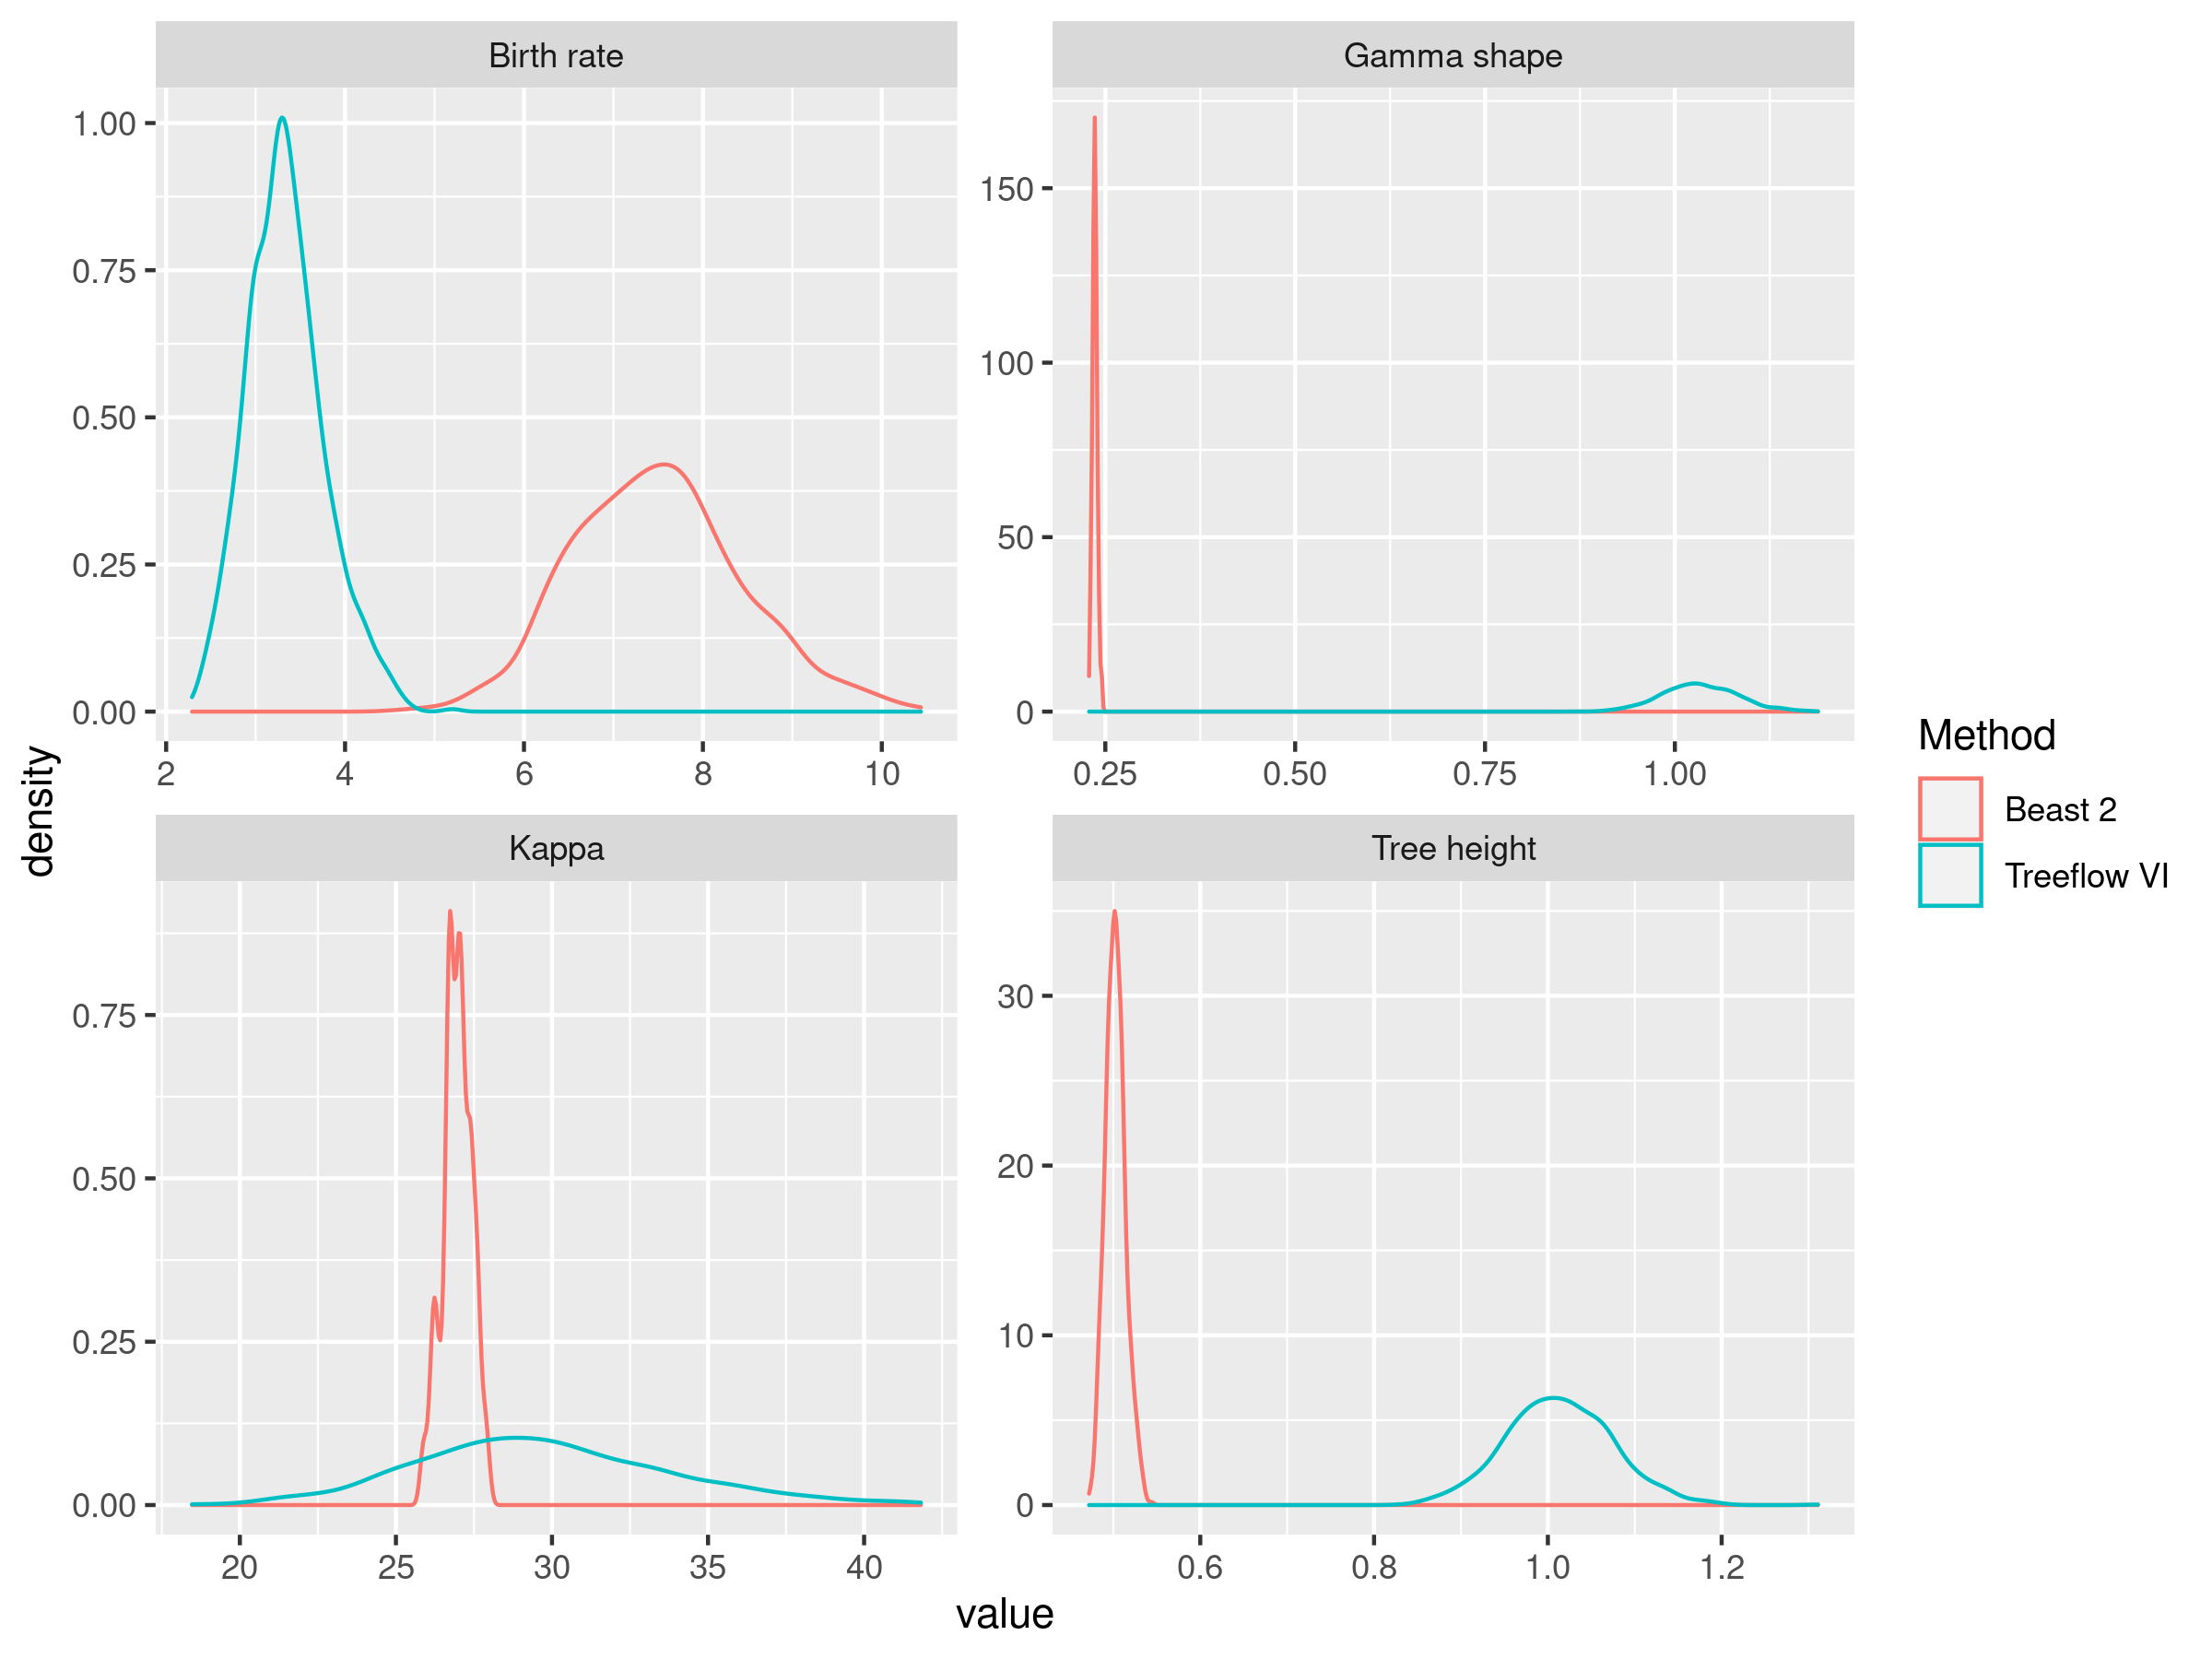
\includegraphics[width=\linewidth]{manuscript/figures/carnivores-marginals}
    \caption{Carnivores base model posterior marginal parameter estimates}
    \label{fig:carnivoresmarginals}
\end{figure}

This problem could be approached by means of Bayesian model comparison; a lack of preference for a model allowing between-lineage variation of the ratio could indicate that the substitution model lacks the power to separate variation `signal' from saturation `noise'. Firstly, we construct a standard phylogenetic model with a HKY substitution model with a single transition-transversion ratio parameter (\textit{kappa}). We perform inference using ADVI, and also using MCMC as implemented in BEAST 2 \cite{bouckaert2019beast}. Since this model is of the form of a standard phylogenetic analysis, it could be fit using TreeFlow's command line interface. Figure \ref{fig:carnivoresmarginals} compares the marginal parameter estimates obtained from TreeFlow and BEAST 2. The discrepancies in distribution, apparent in the estimates of the frequencies and tree height, can be attributed to the approximation error introduced by ADVI. Most importantly, the estimate of the parameter of interest, kappa, appears reasonable.

\begin{figure}
    \begin{minted}[highlightlines={19-22,41-44},baselinestretch=0.9,highlightcolor=cyan]{py}
site_category_count = 4
pattern_counts = alignment.get_weights_tensor()
subst_model = HKY()

def build_sequence_dist(tree, kappa, frequencies, site_gamma_shape):
    unrooted_tree = tree.get_unrooted_tree()
    site_rate_distribution = DiscretizedDistribution(
        category_count=site_category_count,
        distribution=Gamma(
            concentration=site_gamma_shape,
            rate=site_gamma_shape
        ),
    )
    transition_probs_tree = get_transition_probabilities_tree(
        unrooted_tree,
        subst_model,
        rate_categories=site_rate_distribution.normalised_support,
        frequencies=frequencies,
        frequencies=tf.broadcast_to(
            tf.expand_dims(frequencies, -2),
            kappa.shape + (4,)
        ),
        kappa=kappa
    )
    return SampleWeighted(
        DiscreteParameterMixture(
            site_rate_distribution,
            LeafCTMC(
                transition_probs_tree,
                expand_dims(frequencies, -2),
            ),
        ),
        sample_shape=alignment.site_count,
        weights=pattern_counts
    )

model = JointDistributionNamed(dict(
    birth_rate=LogNormal(c(1.0), c(1.5)),
    tree=lambda birth_rate: Yule(tree.taxon_count, birth_rate),
    kappa=LogNormal(c(0.0), c(2.0)),
    kappa=Sample(
        LogNormal(c(0.0), c(2.0)),
        tree.branch_lengths.shape
    ),
    site_gamma_shape=LogNormal(c(0.0), c(1.0)),
    frequencies=Dirichlet(c([2.0, 2.0, 2.0, 2.0])),
    sequences=build_sequence_dist
))
    \end{minted}
    \label{fig:carnivorescode}
    \caption{Code to specify models for carnivores analysis. Highlighted lines show changes (from previous line) to add kappa variation across lineages.}
\end{figure}

We then altered this model to estimate a separate ratio for every lineage on the tree; the implementation of this was simple and scalable as a result of TensorFlow's vectorization and broadcasting functionality. We compare the models using estimates of the marginal likelihood \cite{mackay2003information}. The \textit{marginal likelihood}, or \textit{evidence}, the integral of the likelihood of the data over model parameters, is typically analytically intractable and challenging to compute using MCMC methods \cite{xie2011improving}. The closed-form approximation to the posterior distribution provided by variational inference means we can easily estimate the marginal likelihood using importance sampling, a utility provided by TreeFlow. This corrects for some of the posterior approximation error described above.

\begin{figure}
    \centering
    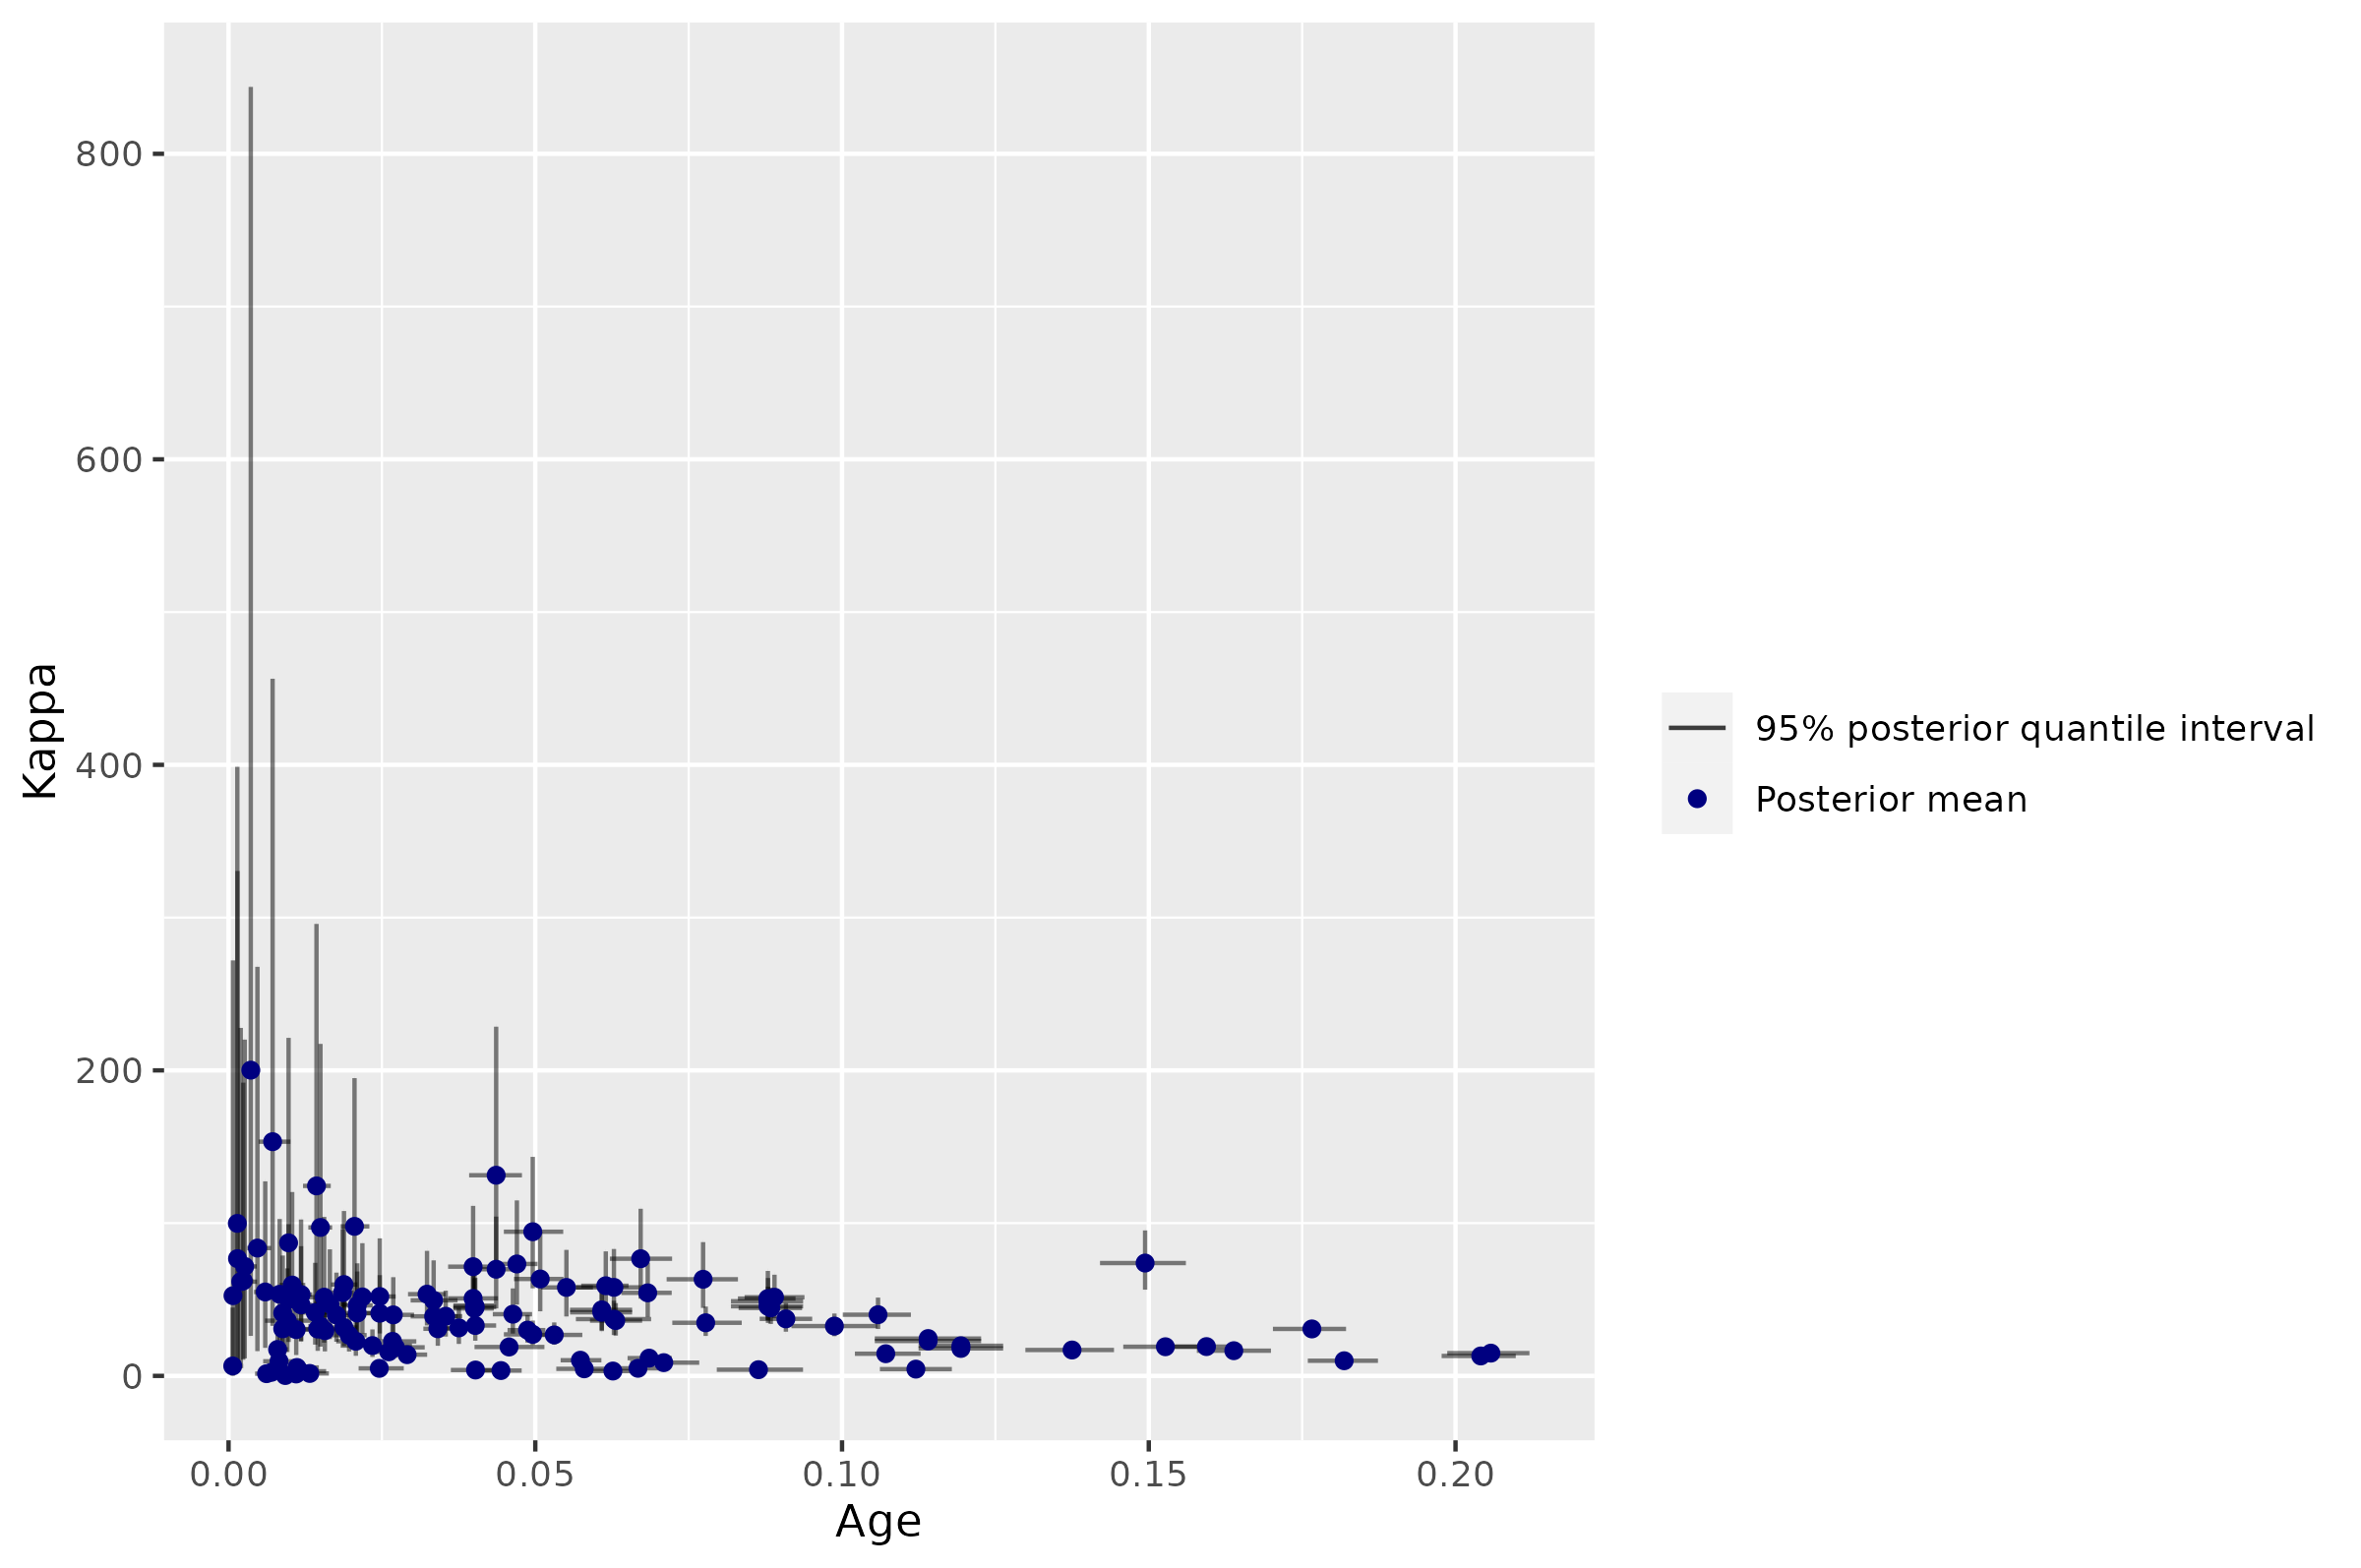
\includegraphics[width=\linewidth]{manuscript/figures/carnivores-kappa}
    \caption{Lineage age (number of expected substitutions per site before the present) vs estimated transition/tranversion ratio (Kappa) for carnivores dataset}
    \label{fig:carnivoreskappa}
\end{figure}

\begin{figure}
    \centering
    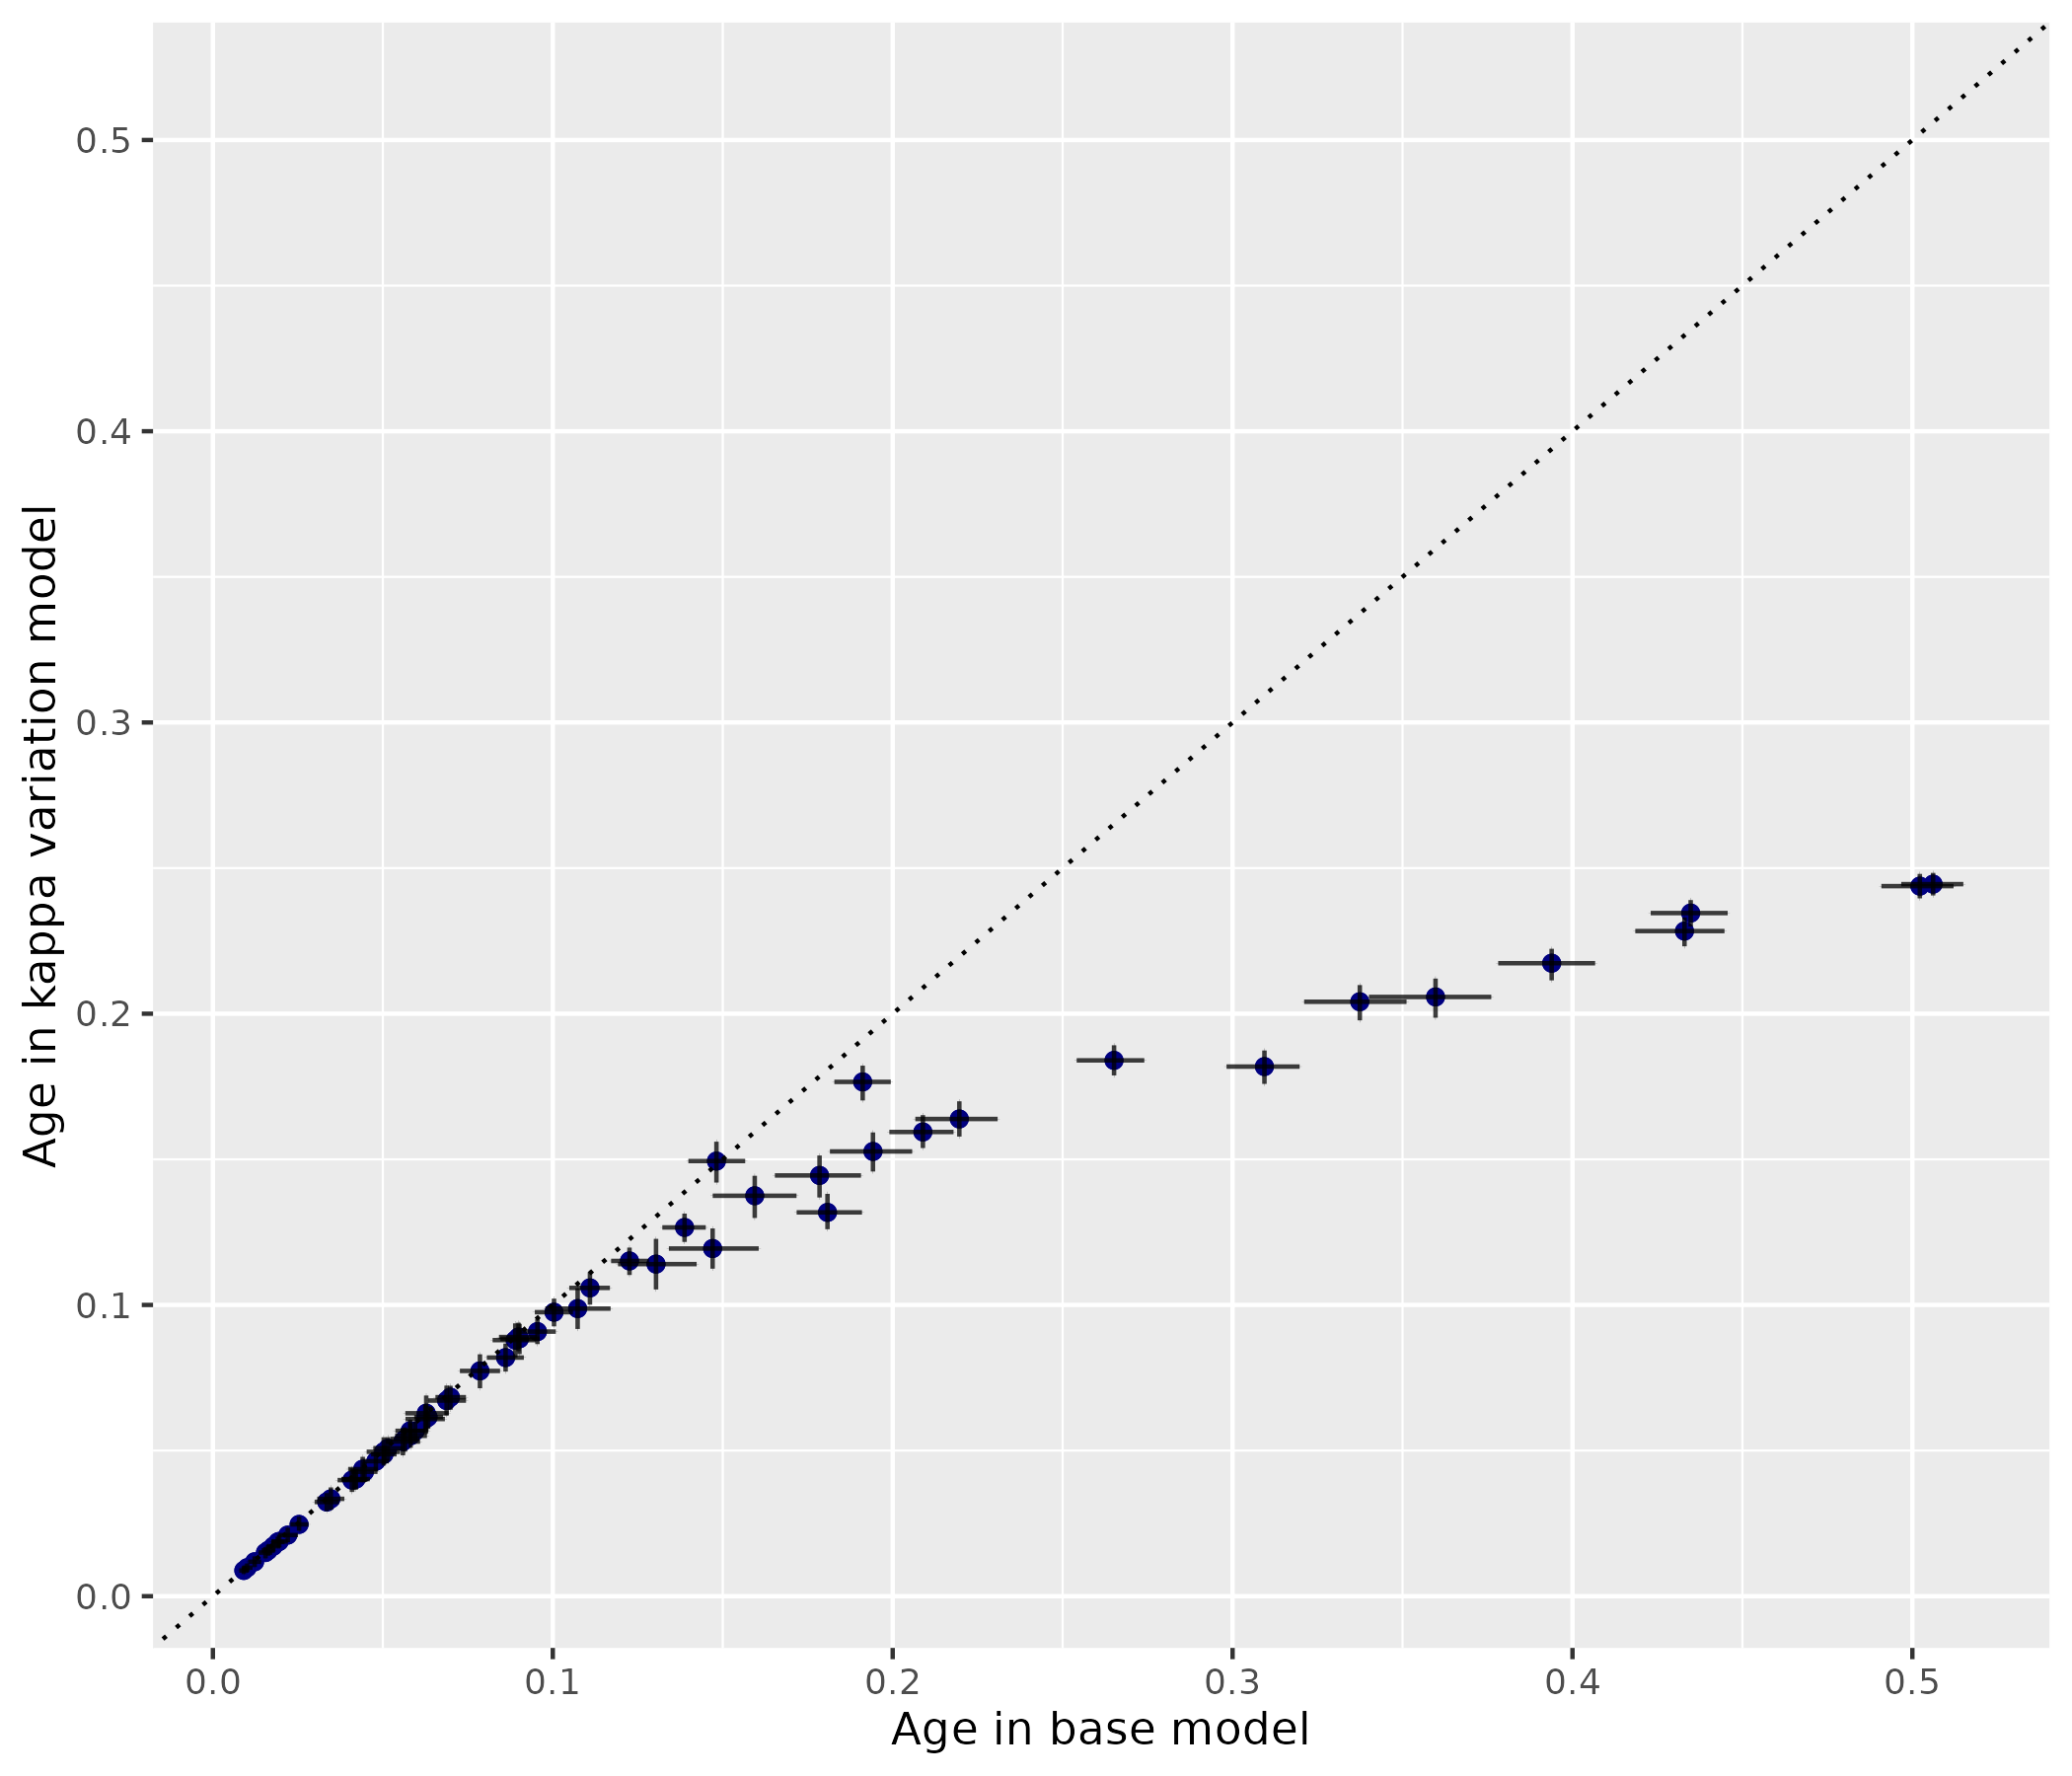
\includegraphics[width=\linewidth]{manuscript/figures/carnivores-model-trees}
    \caption{Node age estimates for base model vs per-lineage kappa variation model}
    \label{fig:carnivorestree}
\end{figure}

The estimated per-lineage kappa parameters are shown in Figure \ref{fig:carnivoreskappa}. Kappa estimates decline with the age of the lineage, which agrees with the results of the previous studies. The marginal likelihood for the model with transition-transversion ratio variation across lineages was higher than for the base model. This means that, under the other components of this model, the data supports variation in the ratio. This does not necessarily imply that transition-transversion ratio in the true generative process of the data varies in the same way, but could be a useful consideration in designing more sophisticated models of nucleotide substitution. The growth in uncertainty in kappa estimates deeper in the tree supports previous conclusions that nucleotide substitution models are unable to effectively estimate the number of substitutions on older branches \cite{duchene2015declining}. Figure \ref{fig:carnivorestree} shows that the kappa variation model shortens older branches, leading to a substantially reduced overall tree height estimate, with proportionally similar uncertainty in node height estimates. This is not a proper dating analysis as it does not consider uncertainty in the mutation rate and is not time-calibrated, but it is clear that this model could significantly affect time estimates.

\begin{figure}

    \inputminted{yaml}{out/h3n2/model.yaml}

    \caption{YAML model definition for the analysis of the influenza dataset}
    \label{fig:fluyaml}
\end{figure}

\begin{figure}
    \centering
    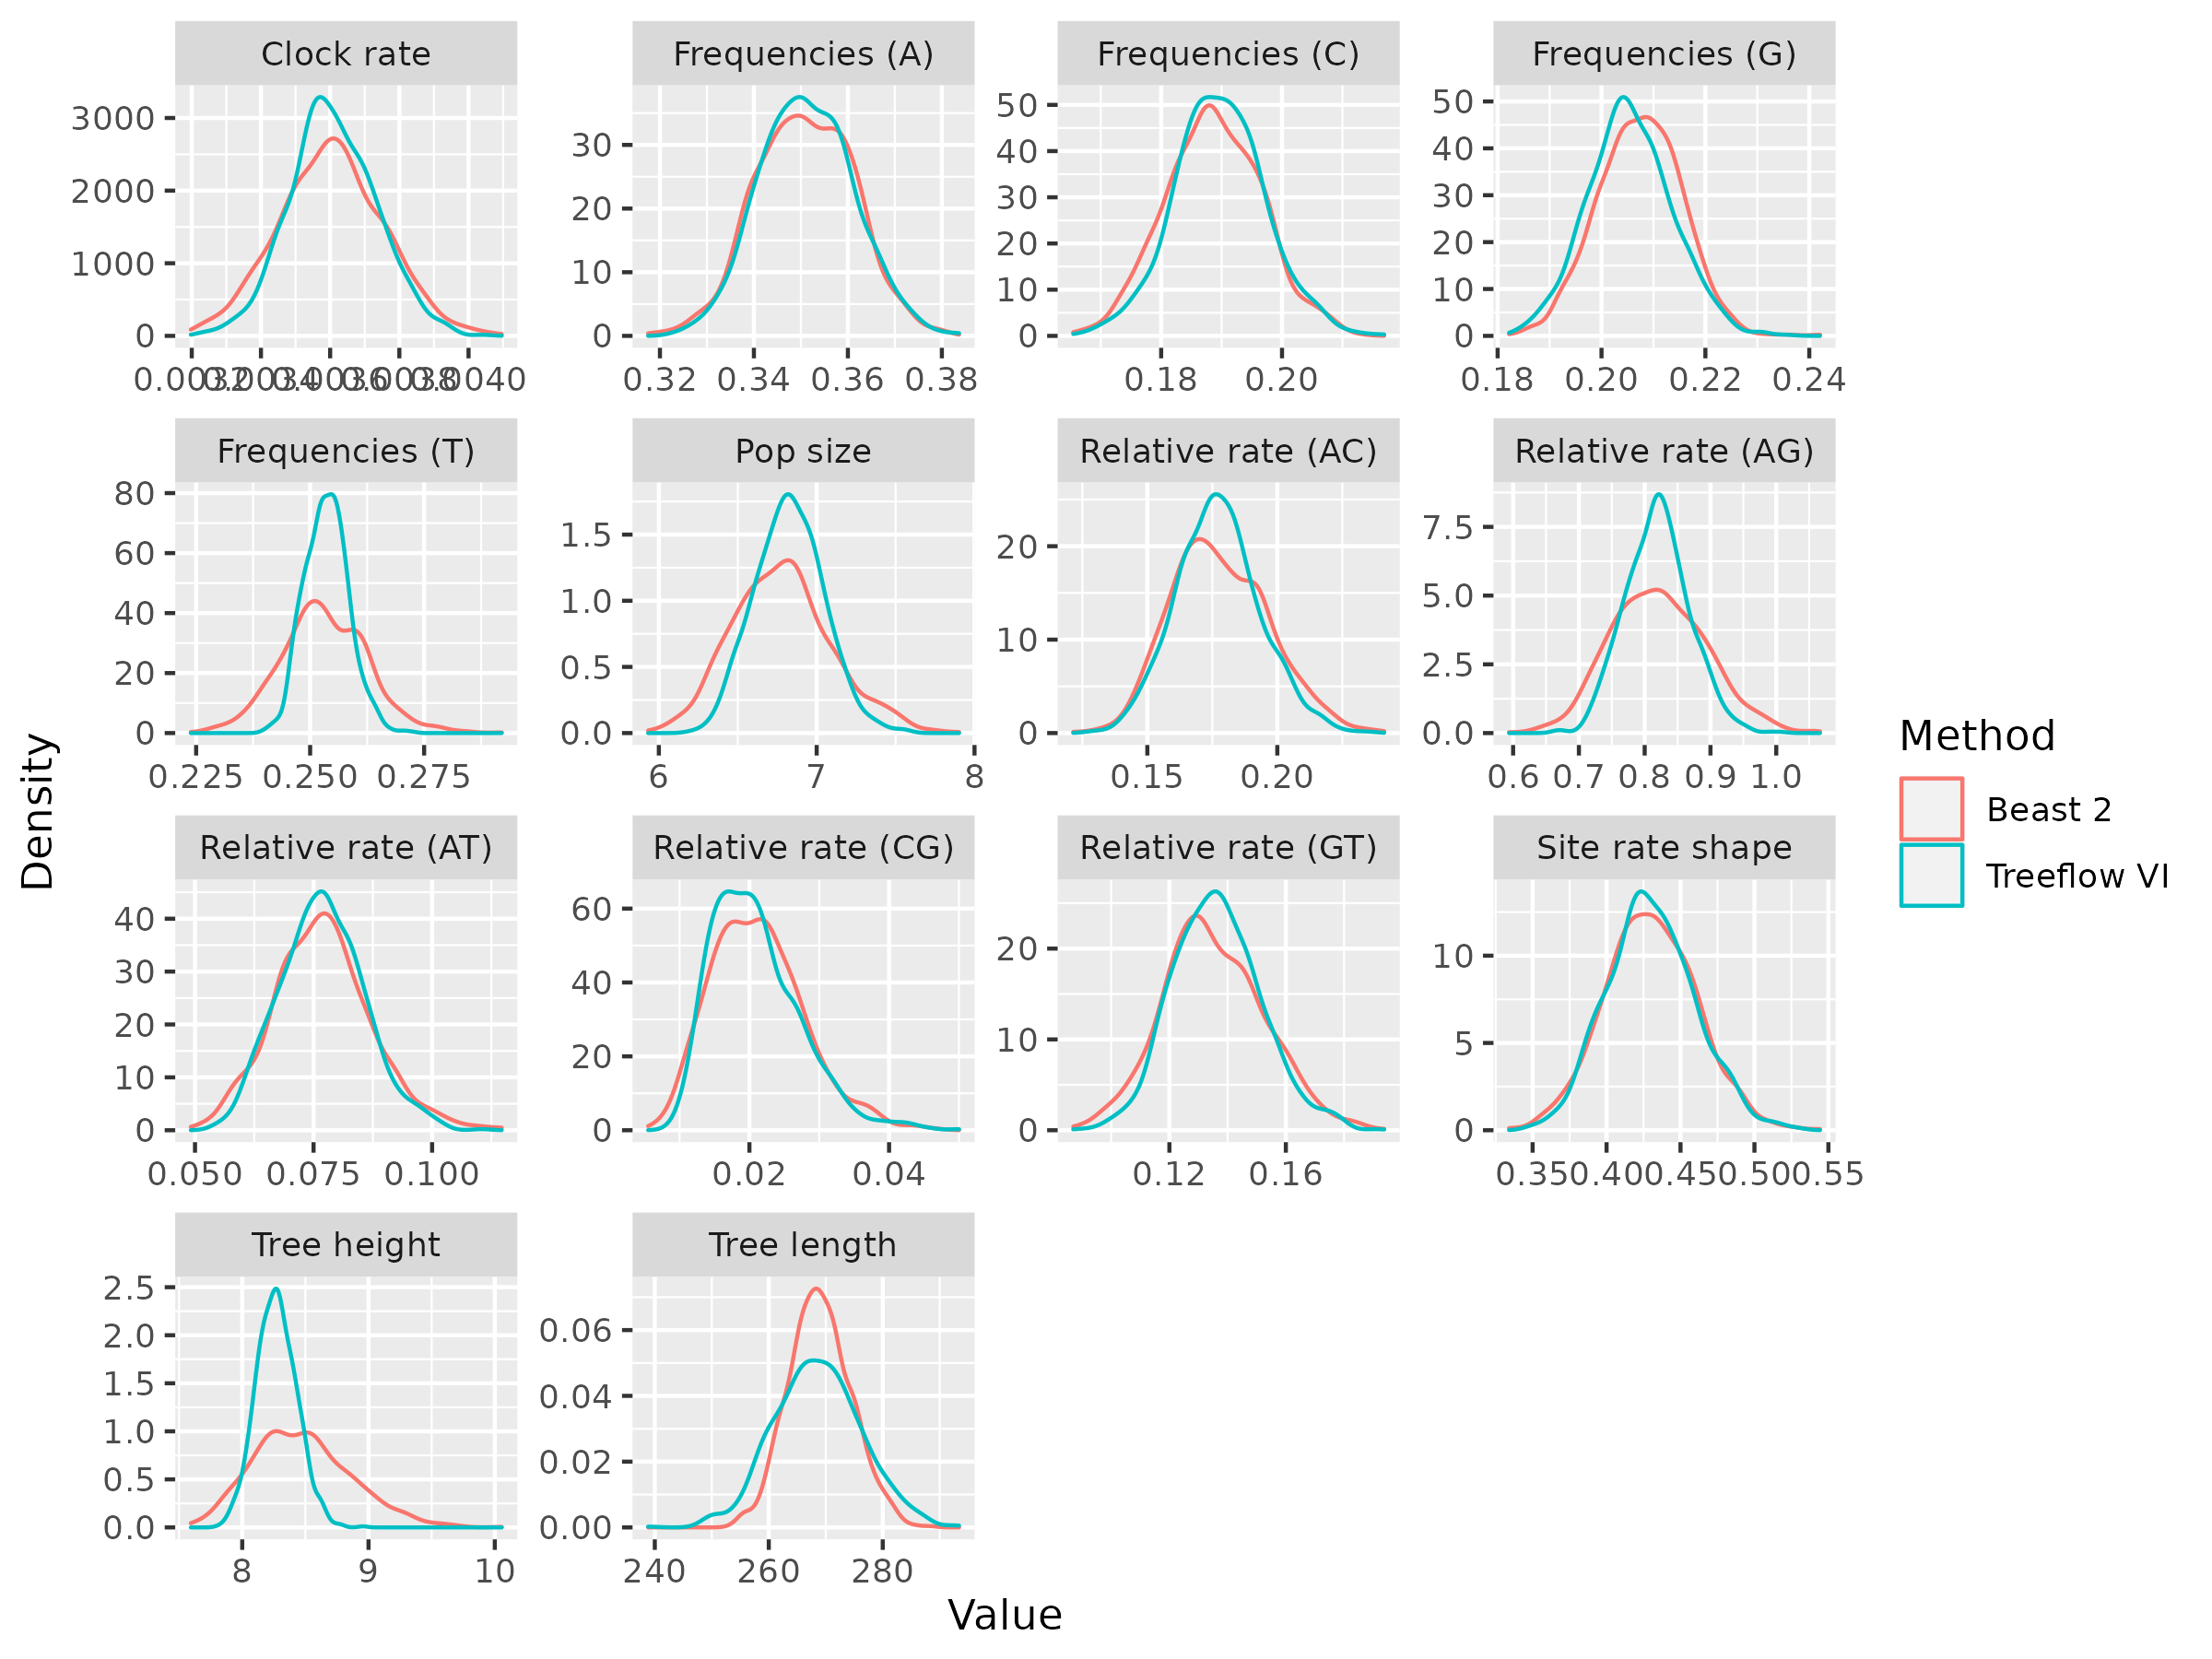
\includegraphics[width=\linewidth]{manuscript/figures/h3n2-marginals}
    \caption{Influenza parameter marginal posterior distributions}
    \label{fig:flumarginals}
\end{figure}

\begin{figure}
    \centering
    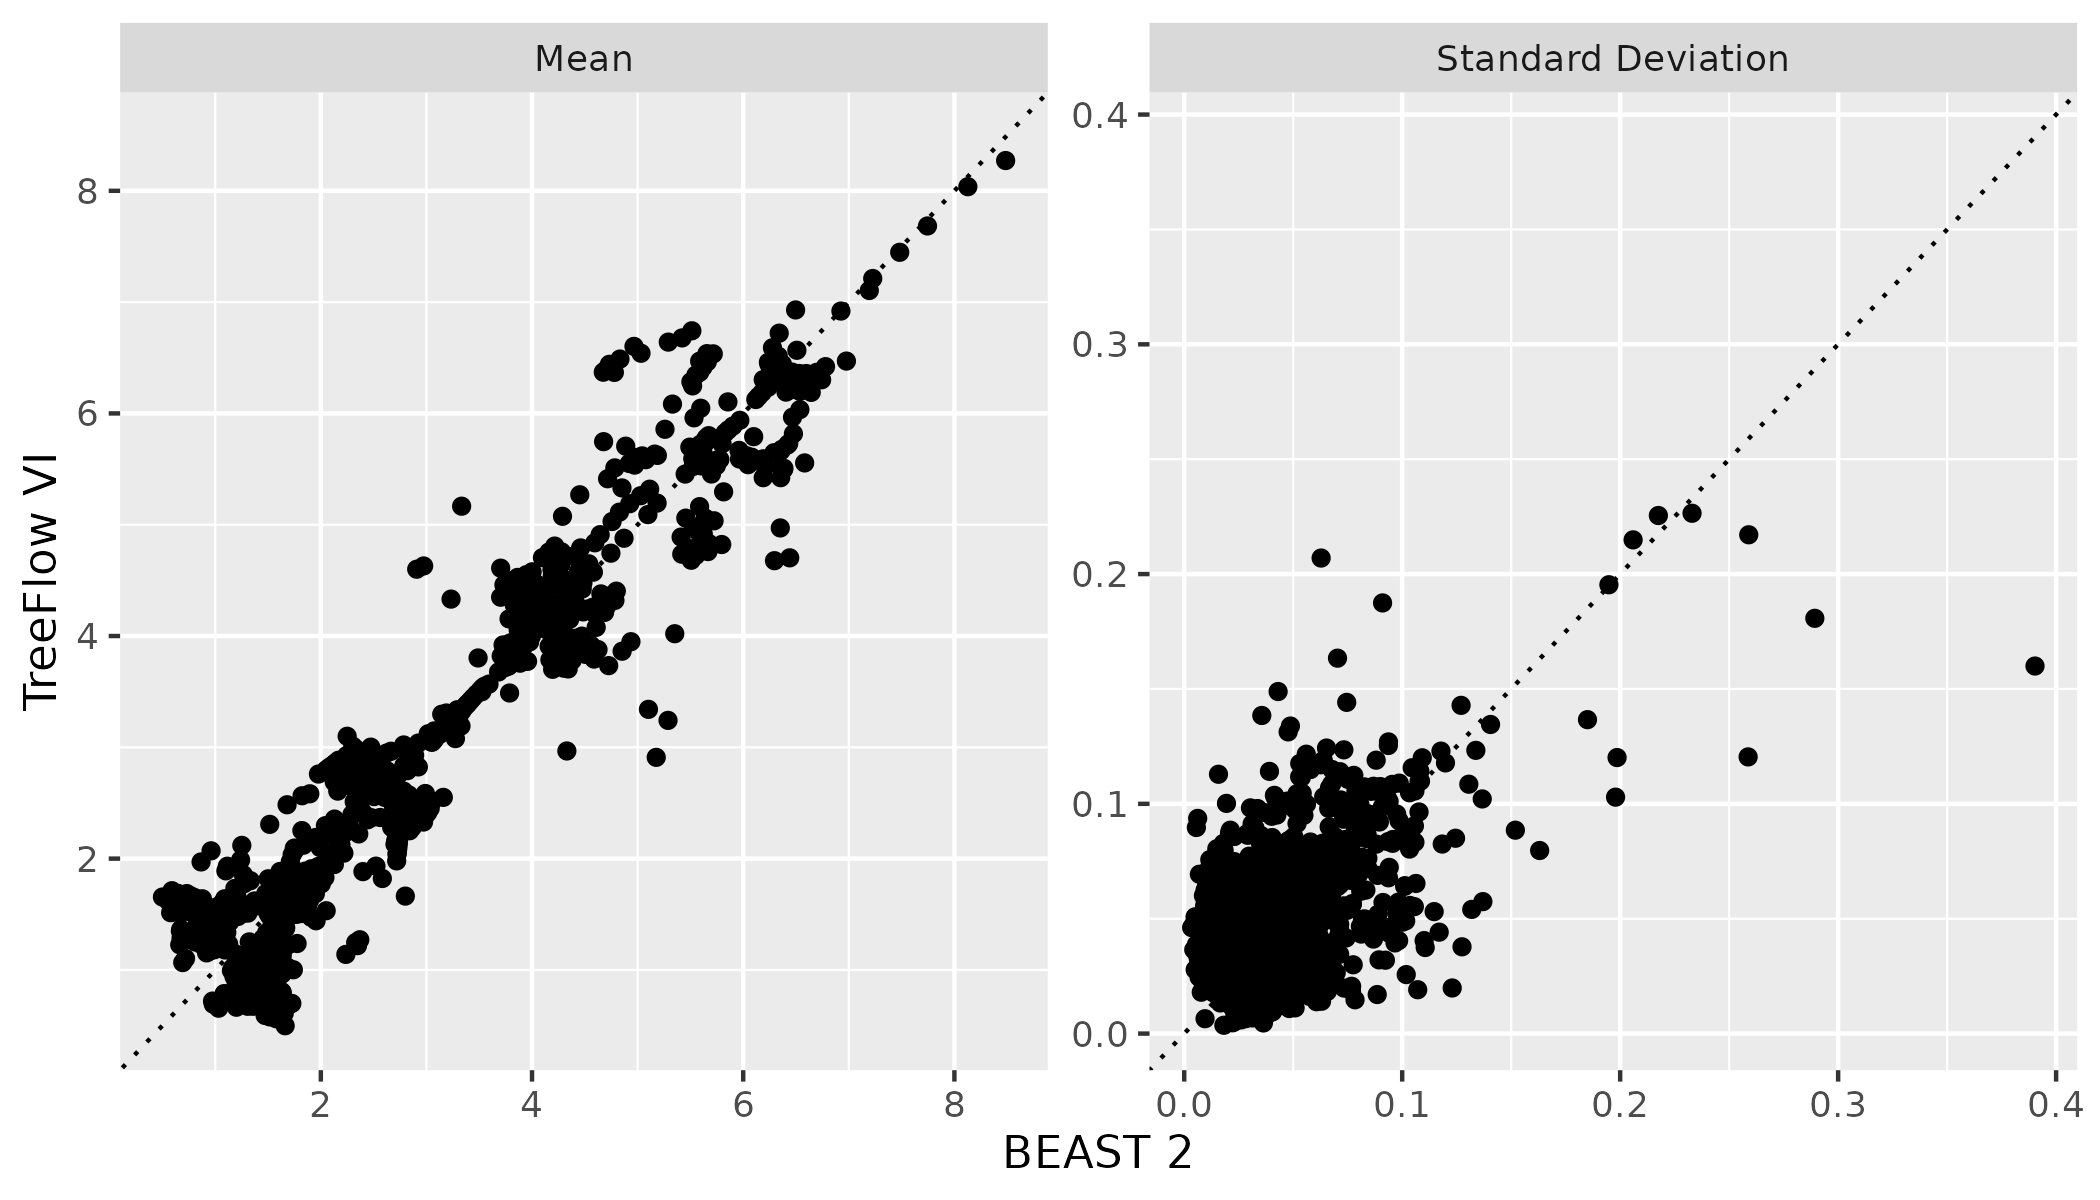
\includegraphics[width=\linewidth]{manuscript/figures/h3n2-trees}
    \caption{Influenza node height posterior distribution statistics}
    \label{fig:flutree}
\end{figure}

\subsection{Scalable inference}

In the analysis of the 980-taxon influenza dataset, we demonstrate the scalability of variational inference. We performed variational inference using TreeFlow's command line interface. The model used for inference included a coalescent prior with a constant population size on the tree, a strict molecular clock, a discretized Gamma model of site rate variation and a GTR substitution model. The YAML model definition code for this model, including parameter priors, is shown in Figure \ref{fig:fluyaml}. This parameterization of the GTR substitution model (here named \texttt{gtr\_rel}), with independent priors on five of the relative rates and one held fixed to 1, is used to allow comparison of parameter estimates with BEAST 2. It is also possible to use a six-rate GTR parameterisation with a Dirichlet prior in TreeFlow.

Figure \ref{fig:flumarginals} shows the marginal parameter estimates obtained from this dataset, compared to those obtained from a fixed-topology MCMC analysis using BEAST 2. The posterior distributions of most parameters are approximated with high fidelity by the mean field approximation. The uncertainty in the tree height, coalescent effective population size, and clock rate are slightly underestimated. This is a result of using an approximation that ignores the correlations between these parameters that are present in the posterior.

Figure \ref{fig:flutree} compares the divergence time estimates. TreeFlow's mean field variational approximation assumes the posterior distribution on the times of the tree are independent Normal distributions transformed through the node height ratio transformation to respect the time constraints of the tree. However, the true posterior is almost certainly not of this form, so the approximation introduces error. In general, the mean of the posterior distribution is well approximated, in particular for the oldest seven nodes of the tree. The posterior means of other divergence times are generally close but not identical to the true posterior. The error is more apparent in the posterior uncertainty; the standard deviation estimates produced by variational inference often differ substantially from the true posterior. While mean field variational inference seems effective for estimating the parameters of the phylogenetic model the estimates of divergence times appear less reliable. Variational approximations that better capture the form of the true posterior would improve the quality of these estimates.

BEAST 2 MCMC sampling was run for 30,000,000 iterations. Convergence was checked using effective sample size, which was computed for all parameters using ArviZ \cite{kumar2019arviz}. Multiple runs were performed to tune MCMC operator weights to improve ESSs. Generally, the minimum acceptable ESS is 100, though 200 is preferred \cite{drummond2015bayesian}. The analysis resulted in a minimum effective sample size of 125. The wall clock runtime for the BEAST 2 analysis was 5 hours and 57 minutes. The TreeFlow analysis converged in 20,000 iterations which took 3 hours and 3 minutes. This shows that variational inference has favourable scaling for large phylogenetic datasets despite the more expensive gradient computations required, and that TreeFlow's slower phylogenetic likelihood implementation performs well enough to be useful in real-world inference scenarios.

\section{Benchmarks}

The phylogenetic likelihood is the computation that dominates the computational cost of model-based phylogenetic inference. We benchmark the performance of our TensorFlow-based likelihood implementation against specialized libraries. Since gradient computations are of equal importance to likelihood evaluations in modern automatic inference regimes, we also benchmark computation of derivatives of the phylogenetic likelihood, with respect to both the continuous elements of the tree and the parameters of the substitution model. A clear difference emerges in the implementation of derivatives; TreeFlow's are based on automatic differentiation while bespoke libraries need analytically-derived gradients. Therefore, we do not necessarily expect our implementation to be as fast as bespoke software, but it does not rely on analytical derivation of gradient expressions for every model and therefore automatically supports a wider range of models.

We compare the performance of TreeFlow's likelihood implementation against BEAGLE \cite{ayres2019beagle}. BEAGLE is library for high performance computation of phylogenetic likelihoods. Recent versions of BEAGLE implement analytical gradients with respect to tree branch lengths \cite{ji2020gradients}. We use BEAGLE via the \texttt{bito} software package \cite{bito}, which provides a Python interface to BEAGLE and also numerically computes derivatives with respect to substitution model parameters using a finite differences approximation.

We also compare TreeFlow with a simple likelihood implementation \cite{phylojax} based on another automatic differentiation framework, JAX \cite{jax2018github}. In contrast to TensorFlow's function mode, which the benchmarked TreeFlow implementation uses, JAX uses an eager execution model and is compatible with native Python control flow.

Benchmarks are performed on simulated data. Simulation allows the generation of a large number of data replicates with appropriate properties. Since we want to investigate the scaling of likelihood and gradient calculations with respect to the number of sequences, we simulate data for a range of sequence counts. Sequence counts are selected as increasing powers of 2 to better display asymptotic properties of the implementations. We simulate data with sequence counts ranging from 32 to 2048. Trees are simulated under a coalescent model for a given number of taxa, and then nucleotide sequences of length 1000 are simulated under a fixed rate of evolution and a HKY substitution model. Tree and sequence simulations are performed using BEAST 2 \cite{bouckaert2019beast}.

We benchmark 4 distinct computations on these datasets. Firstly, for each replicate we compute the phylogenetic likelihood under a very simple model of sequence evolution. This uses a Jukes-Cantor model of nucleotide substitution and no model of site rate variation. Secondly, we calculate derivatives with respect to branch lengths under this simple model. Thirdly, we compute the likelihood under a more sophisticated substitution model, with a discretized Weibull distribution with 4 rate categories to model site rate variation and a GTR model of nucleotide substitution. We selected the Weibull distribution for site rate variation since it is implemented in \texttt{bito}. Finally, we compute derivatives with respect to both branch lengths and the parameters of the substitution model (the 6 GTR relative substitution rates, 4 base nucleotide frequencies, and the Weibull site rate shape parameter). Each computation is performed 100 times on 10 simulated datasets.


\begin{figure}
    \centering
    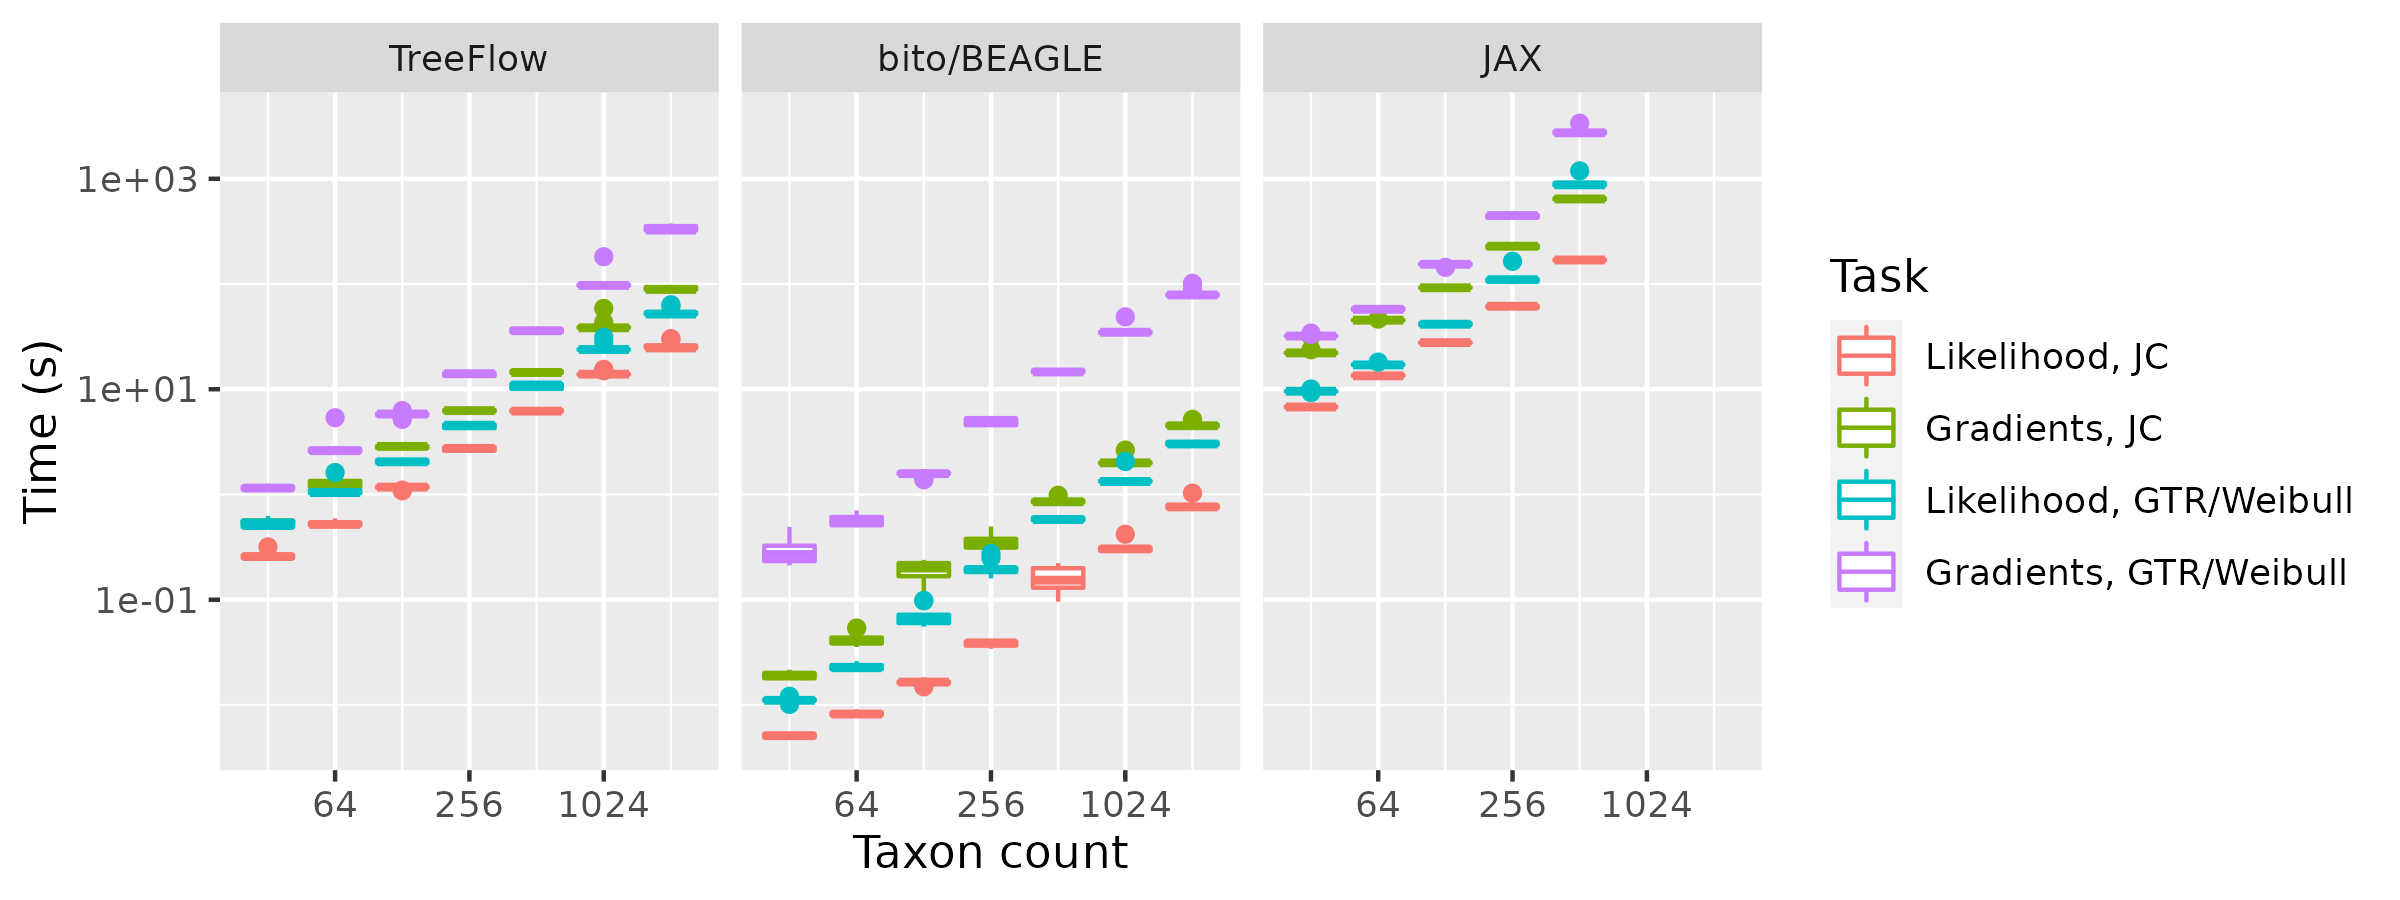
\includegraphics[width=\linewidth]{manuscript/figures/benchmark-log-scale-plot}
    \caption{Times from phylogenetic likelihood benchmark (100 evaluations for 1000 sites)}
    \label{fig:benchmark}
\end{figure}

\begin{table}
    \centering
    \begin{tabular}{lllrr}
\toprule
 &  &  & Mean time (512 taxa) & log-log slope \\
Model & Computation & Method &  &  \\
\midrule
\multirow[t]{6}{*}{JC} & \multirow[t]{3}{*}{Likelihood} & TreeFlow & 6.23 & 1.13 \\
 &  & bito/BEAGLE & 0.16 & 1.27 \\
 &  & JAX & 168.79 & 1.15 \\
 & \multirow[t]{3}{*}{Gradients} & TreeFlow & 14.55 & 1.23 \\
 &  & bito/BEAGLE & 0.87 & 1.33 \\
 &  & JAX & 644.22 & 1.19 \\
\multirow[t]{6}{*}{GTR/Weibull} & \multirow[t]{3}{*}{Likelihood} & TreeFlow & 10.73 & 1.12 \\
 &  & bito/BEAGLE & 0.58 & 1.40 \\
 &  & JAX & 908.24 & 1.58 \\
 & \multirow[t]{3}{*}{Gradients} & TreeFlow & \bfseries 36.14 & \bfseries 1.34 \\
 &  & bito/BEAGLE & \bfseries 14.74 & \bfseries 1.41 \\
 &  & JAX & \bfseries 2801.35 & \bfseries 1.58 \\
\bottomrule
\end{tabular}

    \caption{Results of phylogenetic likelihood benchmark. Times for gradients for the GTR/Weibull are highlighted as they are the most relevant computation for gradient-based inference on real data.}
    \label{tab:benchmarkfit}
\end{table}

Figure \ref{fig:benchmark} shows the results of the benchmarks with a log scale on both axes. For likelihood computation with both models and branch gradient computation with the simple model \texttt{bito}/BEAGLE are at least an order of magnitude faster than TreeFlow. This is expected as BEAGLE is a highly optimized special-purpose library written in native code. The performance gap grows much smaller for computing the gradients of the more complex substitution model. \texttt{bito} performs at least 2 likelihood evaluations for each additional parameter when calculating the gradient with respect to substitution model parameters, while the overhead for substitution model parameters with automatic differentiation is minimal. We expect TreeFlow to surpass \texttt{bito}/BEAGLE for substitution models with even more parameters (e.g. amino acid substitution models \cite{adachi1996model}), or those where the number of parameters grows with the number of sequences, as in the example below.

For typical real-world phylogenetic analyses, a model with many parameters, such as the GTR/Weibull model in our benchmarks, is used. For modern Bayesian inference methods such as variational inference and Hamiltonian Monte Carlo, the gradient is the primary computation performed at each iteration. We observe that TreeFlow's times for this combination of model and computation are within an order of magnitude of \texttt{bito}/BEAGLE's, around 2-3 times slower. Therefore for applied analyses the automatic differentiation-based computations of TreeFlow presents a reasonable alternative to specialized software while similtaneously offering greater flexibility.

We also observe that the runtimes for TreeFlow are roughly an order of magnitude less than those of the JAX-based implementation. These indicate that the control flow constructs and execution model of TensorFlow are a good choice for implementing tree-based computations compared to the eager execution model of JAX.

Table \ref{tab:benchmarkfit} shows the coefficients obtained from fitting a linear model to the benchmark times where the predictor is the log-transformed number of sequences and the target is the log-transformed runtime. The slope parameter estimates from these fits is a rough empirical estimate of the polynomial degree of the computational scaling. The slope parameters for all TreeFlow computations are well below 2 and indicate a roughly linear scaling with the size of the data. For the JC benchmark, the only gradients computed are with respect to branch lengths, so the whole computation for \texttt{bito}/BEAGLE is the analytical linear-time branch gradient. TreeFlow's scaling is certainly not worse in this case, indicating that the TensorArray-based likelihood implementation enables linear-time branch gradients.


\section{Discussion}

The combination of flexibility and scalability of libraries like TreeFlow has the potential to be useful for rapid analysis of large modern genetic datasets, such as those assembled for tracking infectious diseases \cite{hadfield2018nextstrain}. For this purpose, TreeFlow's true power would be unlocked with the implementation of improved modelling and inference tools for evolutionary rates and population dynamics.

For principled dating analyses, uncertainty in evolutionary rate parameters must be considered. Posterior distributions involving these parameters may have significant correlation structure which would be ignored by variational inference using a mean-field posterior approximation. These parameters typically receive special treatment in MCMC sampling routines \cite{drummond2006relaxed, zhang2020improving}. As observed in our analysis on the influenza dataset, the mean field approximation fails to accurately capture the posterior distribution on all internal divergence time estimates. Implementing structured posterior approximations for these models could substantially improve the reliability of parameter estimates obtained using variational inference while scaling to extremely large datasets.

Additionally, implementing flexible models for population dynamics, such as nonparametric coalescent models \cite{drummond2005bayesian, minin2008smooth, gill2013improving}, could provide valuable insights from large datasets. These models would result in complex posterior distributions, which would need to be accounted for in a variational inference scheme. If these coalescent models could be made to work effectively in TreeFlow, the probabilistic programming paradigm would allow for rapid computational experimentation with novel models of time-varying population parameters.

Finally, the most significant functionality for phylogenetic inference missing from TreeFlow is inference of the tree topology. TreeFlow's tree representation could allow for the topology to become an estimated parameter, such as in existing work on variational Bayesian phylogenetic inference \cite{zhang2018variational}. Efficiently implementing the computations required for these algorithms in the TensorFlow framework would certainly be a major computational challenge.

\section{Conclusion}

TreeFlow is a software library that provides tools for statistical modelling and inference on phylogenetic problems. Probabilistic programming provides flexible model definition involving phylogenetic trees and molecular sequences, and automatic differentiation enables the application of modern scalable inference algorithms. TreeFlow's automatic differentiation-based implementations of core gradient computations provide reasonable performance compared to specialized phylogenetic libraries. These building blocks have the potential to be used in valuable phylogenetic analyses of large and complex genetic datasets.

\section{Availability}

TreeFlow is an open-source Python package. Instructions for installing TreeFlow, and examples of using it as a library and command line application can be found at \url{https://github.com/christiaanjs/treeflow}.

\section{Supplementary material}

Datasets, model definitions, starting values, and BEAST 2 XML files used in the biological examples are available at \url{https://github.com/christiaanjs/treeflow-paper/releases/tag/v0.0.1}.


%If you have any acknowledgements, please include them here.
%\section{Acknowledgements}

%If your paper has accompanying supplementary data, please include the below statement in your PDF.
%\section{Supplementary Material}
%Data available from the Dryad Digital Repository:
% \href{http://dx.doi.org/10.5061/dryad.[NNNN]}%
% {http://dx.doi.org/10.5061/dryad.[NNNN]}.
%\url{http://dx.doi.org/10.5061/dryad.[NNNN]}.

\bigskip\bigskip

% REFERENCES

% The best way to enter references is to use BibTeX.
\bibliography{main}

% Alternatively you could enter them by hand, like this:

% 1. All authors should be listed i.e. no use of et al.
% 2. Dashes should not be used to replace author names in repeat entries

% Please include any figure captions on a separate page after the references. Figures themselves should be embedded in the text.

%\begin{figure}[!p]
%\centering\includegraphics{fig1}
%\caption{Figure caption}
%\label{Fig1}
%\end{figure}


%\begin{table}[!p]
% 1. Table titles should be in caps and lowercase
% 2. Footnotes can be used in Tables (a,b,c)}
%\tblcaption{Table title
%\label{Table1}}
%{\tabcolsep=4.25pt
%\begin{tabular}{@{}cccccccccc@{}}
%\tblhead{Heading & Heading & Heading & Heading & Heading}
%Value & Value & Value & Value & Value 
%\lastline
%\end{tabular}}
%\end{table}

%If you have any print appendices, please include them at the end of the document.

\end{document}